\subsection{CodeBo Unplugged: Um jogo desplugado para o ensino de Pilha}

Foi desenvolvido o jogo de tabuleiro \textit{CodeBo unplugged} com o intuito de ensinar a estrutura de dados Pilha a alunos do ensino fundamental de forma lúdica, utilizando elementos como robôs e mapas que aumentam em dificuldade de forma progressiva. \cite{de2023codebo}

\begin{figure}[H]
	\centering
	\caption{Foto do tabuleiro de CodeBô Unplugged}
	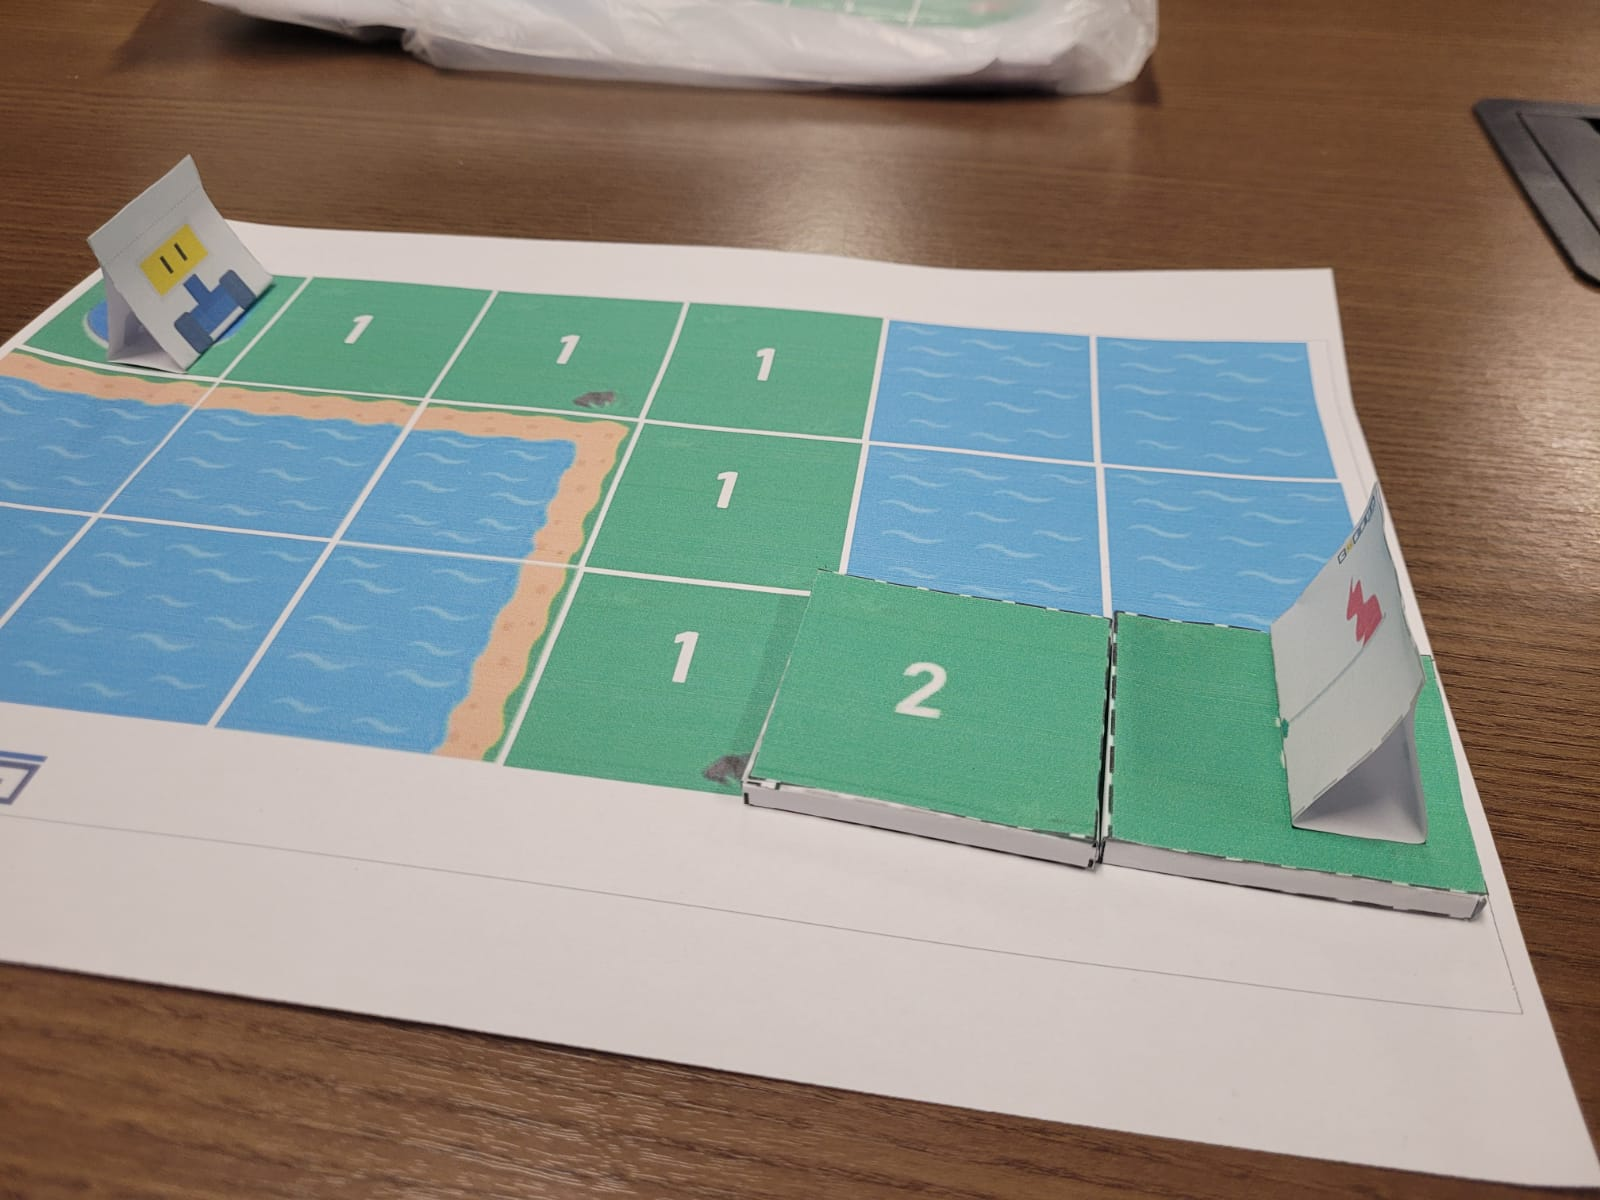
\includegraphics[width=0.8\textwidth]{images/code-unplugged.png}
	\legend{Fonte: \cite{de2023codebo}}
	\label{fig:codebo_unplugged}
\end{figure}

